\documentclass[11pt,a4paper,headsepline,hidelinks]{scrreprt} % KOMA-Script
\usepackage[italian]{babel}
\usepackage[utf8]{inputenc}
\usepackage[T1]{fontenc}
\usepackage{graphicx}
\usepackage{amsfonts}
\usepackage{hyperref}
\pagestyle{headings}
\renewcommand{\arraystretch}{1.5}

\begin{document}
    \title{Relazione di stage - Bozza}
	\subject{Analisi e progettazione di un'interfaccia grafica per la consultazione dei contenuti informativi in una piattaforma web tematica}
    \author{Nicola Moretto (matr. 578258)}
    \date{\today}

    \maketitle

	\tableofcontents

	\listoffigures
	\begingroup
	\let\clearpage\relax
	\listoftables
	\endgroup

	% CHAPTER
	\chapter{Introduzione}
	\label{ch:tesi:intro}

	\section{Contenuti}
	Il presente documento costituisce una relazione dettagliata in merito all'attività di stage svolta dallo studente Nicola Moretto presso l'azienda \textit{Sintesi Srl}. I contenuti sono organizzati nei seguenti capitoli:
	\begin{description}
	  \item[\nameref{ch:tesi:intro}] \hfill \\
	  Il primo capitolo illustra brevemente la struttura del documento e le convenzioni tipografiche utilizzate.
	  \item[\nameref{ch:tesi:azienda}] \hfill \\
	  \ldots
	  \item[\nameref{ch:tesi:progetto}] \hfill \\
	  \ldots
	  \item[\nameref{ch:tesi:stage}] \hfill \\
	  \ldots
	  \item[\nameref{ch:tesi:valutazioni}] \hfill \\
	  \ldots
	  \item[\nameref{ch:appendice:glossario}] \hfill \\
	  \ldots
	\end{description}

	\section{Convenzioni tipografiche}
	Al fine di agevolare la consultazione del documento, sono state adottate alcune convenzioni tipografiche illustrate di seguito.
	
	\paragraph{Glossario} Gli acronimi, le abbreviazioni, i nomi propri e i termini specialistici contenuti nel presente documento sono illustrati nel \textit{\nameref{ch:appendice:glossario}}, consultabile in appendice, al fine di agevolare la lettura e la comprensione degli argomenti trattati.	La prima occorrenza di ciascun termine o espressione presente nel glossario è riconoscibile per la \underline{sottolineatura}.
	
	\paragraph{Terminologia} I termini propri o di provenienza straniera divenuti di uso corrente nella lingua italiana sono evidenziati in \textit{corsivo}, mentre le parole o espressioni di particolare rilevanza o significato nel presente contesto sono evidenziate in \textsc{maiuscoletto}.
	
	\paragraph{Codice e formule} I nomi di tabelle, classi, package, \ldots sono riportati con un carattere di tipo \textsf{sans serif}, mentre i frammenti di codice o formule sono riconoscibili per l'impiego di un carattere a \texttt{spaziatura fissa}.

	% CHAPTER
	\chapter{L'azienda}
	\label{ch:tesi:azienda}
	L'attività di stage si è svolta presso l'azienda \textit{Sintesi Srl}, operante nel settore IT (\textit{Information Technology}) grazie alla vendita e assistenza di software gestionali proprietari rivolti ad aziende attive nel settore alberghiero.

	Si tratta di una piccola realtà imprenditoriale a clientela nazionale con sede unica a Mestre (VE), la cui gestione e amministrazione è affidata al solo fondatore, che ha assunto il ruolo di tutor esterno e referente aziendale per l'intera durata dello stage.

	Le attività svolte si inseriscono nell'ambito di un progetto esterno rispetto al business dell'azienda e affidato ad un team costituito da differenti figure professionali (sociologi, informatici, ingegneri, \ldots), con le quali sono stati mantenuti regolari contatti al fine di garantire il tempestivo soddisfacimento delle propedeuticità inerenti il mio lavoro di stage e per coordinare adeguatamente le reciproche attività.

	La pianificazione del lavoro in unità settimanali ha decretato lo svolgimento - con identica e regolare cadenza - di incontri con il tutor aziendale aventi lo scopo di:
	\begin{enumerate}
	\item riepilogare le attività svolte nell'arco della settimana;
	\item illustrare e discutere i risultati conseguiti;
	\item fissare gli obiettivi delle attività previste per la settimana successiva.
	\end{enumerate}   

	Le decisioni assunte e le informazioni prodotte nel corso dello stage sono state condivise, discusse e approvate dal suddetto referente, sia in occasione degli incontri pianificati sia - in caso straordinari - nell'arco della settimana.

	% CHAPTER
	\chapter{Il progetto}
	\label{ch:tesi:progetto}
	L'attività di stage svolta presso l'azienda \textit{Sintesi Srl} si inserisce nel quadro di un progetto complesso finalizzato alla realizzazione di una piattaforma web tematica per la condivisione di informazioni e la vendita diretta di prodotti alla clientela.

	\section{Genesi}
	\label{sec:progetto:genesi}
	L'idea di progetto trae origine e ispirazione dalle constatazioni dirette del referente aziendale circa la crisi endemica dei piccoli e medi produttori vitivinicoli, incapaci di sostenere la concorrenza delle grandi realtà industriali sul piano economico e pubblicitario.

	L'impossibilità di offrire i medesimi prezzi al dettaglio e i maggiori costi di gestione connessi alla ridotta scala produttiva hanno contribuito ad aggravare ulteriormente, in un periodo recente caratterizzato da una congiuntura economica sfavorevole, la loro condizione.

	Nello sforzo di cercare una soluzione in grado di risollevarne le sorti, riuscendo a valorizzare la superiore qualità dei prodotti e incrementando al contempo il bacino di clientela, è stato individuato nel rapporto diretto tra produttori e consumatori un elemento chiave, capace di favorirne e sostenerne la ripresa sensibilizzando la clientela (attuale e potenziale) sulla qualità della produzione.

	D'altro canto la formula della vendita diretta di prodotti agroalimentari, che consente di offrire prezzi al dettaglio inferiori grazie all'abbattimento della filiera, ha riscosso un notevole successo negli ultimi anni assumendo forme e connotazioni differenti, come la filosofica dei consumi a \underline{chilometro zero} e i \underline{gruppi d'acquisto}, che sono stati ripresi e sono confluiti nell'idea di progetto pur in una visione e concezione più ampie.

	La scelta di realizzare una piattaforma di \textit{e-commerce}, che sia in grado di raccogliere un vasto numero di utenti interessati alla specifica tipologia di prodotto, è sembrata la naturale risposta al secondo (ma non secondario) obiettivo, ossia l'esigenza di conseguire maggiore visibilità presso la potenziale clientela (locale e nazionale, innanzitutto).

	\section{Reti sociali}
	\label{sec:progetto:reti-sociali}
	Una piattaforma come quella descritta raccoglie consenso e adesione presso gli utenti che manifestano interesse nei confronti di una certa tipologia di prodotti: ciò significa che attorno alla piattaforma tende a costruirsi spontaneamente una \underline{rete sociale}, che può essere definita - dal punto sociologico - come un insieme di persone, aventi interessi in comune e inclini a collaborare e condividere idee o informazioni, e di relazioni di tipo esperienziale definite tra tali soggetti.

	Da tale considerazione scaturisce l'idea di estendere la componente \textit{business} della piattaforma per offrire uno spazio virtuale favorevole alla crescita e al consolidamento della rete sociale, dove coltivare le relazioni sociali attraverso la discussione e la condivisione di conoscenza o esperienza relativa all'area tematica in questione.

	Il modello sociologico di rete sociale non ha riscontro in alcun tipo esistente di piattaforma web per la condivisione di contenuti (blog, forum, \ldots) o di \textit{social network} (Facebook, Twitter, \ldots), in cui il contatto tra soggetti non si traduce o non rispecchia il più delle volte una vera relazione.

	Inoltre diverse piattaforme di condivisione dei contenuti sanciscono una disuguaglianza degli utenti, ove non a tutti coloro che la frequentano è concesso di attingere e contribuire nella stessa misura al patrimonio di conoscenza, ma si assiste ad una scissione tra autori e i fruitori dei contenuti, i primi dei quali acquistano una superiore autorevolezza in virtù del solo ruolo che rivestono.

	Un primo passo fondamentale verso la concretizzazione del modello sociologico di rete sociale consiste nell'abbattimento di ogni distinzione tra creatore e fruitore dei contenuti: l'autorevolezza di ciascun utente si costruisce e si forma nel tempo in base alla qualità dei contenuti pubblicati, anche in considerazione dei giudizi espressi dagli altri utenti.

	Un obiettivo cruciale consiste infine nel trasformare le relazioni virtuali, che si instaurano all'interno della piattaforma web, in vere e proprie relazioni sociali, che si trasferiscono e prosperano nella vita reale.

	% definizione di rete sociale: Granovetter.

	\section{Architettura}
	\label{sec:progetto:architettura}
	Ben presto si individua chiaramente la possibilità di declinare tale modello di piattaforma in innumerevoli varianti, applicabili ai temi più svariati: cucina etnica, moto d'epoca, cinema indipendente, \ldots .

	L'idea di progetto evolve di conseguenza e matura in una piattaforma web tematica, che aspira ad essere costruita intorno alle aspettative e alle esigenze degli utenti e a fondere e coniugare in maniera coerente e consistente due anime:
	\begin{description}
	\item[Business] \hfill \\
	La componente \textit{business} rappresenta un canale di vendita diretto dalle aziende medio-piccole o realtà imprenditoriali indipendenti ai potenziali clienti, corrispondenti all'intero bacino di utenza della piattaforma.
	\item[Social] \hfill \\
	La componente \textit{social} raccoglie il patrimonio conoscitivo ed esperienziale generato dai contributi degli utenti in un serbatoio di conoscenza liberamente accessibile e fruibile.
	\end{description}

	\section{Contenuti informativi}
	\label{sec:progetto:contenuti}
	I contenuti informativi rappresentano il mezzo e lo strumento mediante il quale gli utenti attingono e contribuiscono al patrimonio di conoscenza - riguardante un tema specifico - offerto dalla piattaforma.

	Il processo di individuazione delle classi di contenuti informativi tiene conto essenzialmente delle forme di espressione e di comunicazione tipiche nella vita quotidiana, che a loro volta rispecchiano l'intenzione comunicativa dell'azione compiuta e delle parole espresse da un singolo individuo.

  \paragraph{La metafora dei Lego}
  $$ contenuto informativo = tipo di contenuto + elementi di un contenuto $$

	\section{Criteri di classificazione}
	\label{sec:progetto:classificazione}	

	% CHAPTER
	\chapter{Stage}
	\label{ch:tesi:stage}

	\section{Piano di stage}
	\label{sec:tesi:stage:piano}
		
	%\subsection{Obiettivi e requisiti}
	%\label{sec:tesi:stage:piano:obiettivi}
	L'attività di stage si colloca nell'ambito del progetto presentato nel capitolo \ref{ch:tesi:progetto} perseguendo due obiettivi distinti ma correlati e focalizzandosi sulla componente \textit{social} della piattaforma.
	
		Secondo alcune stime e indagini interne al team di progetto, la piattaforma presenta un potenziale bacino di utenti piuttosto ampio: ci si aspetta dunque che l'attività e le dimensioni (in termini, ad esempio, di numero di contenuti pubblicati) possano attestarsi su livelli tali da imporre valutazioni di carattere tecnico, atte a garantire che il sistema sia in grado di gestire in modo accettabile il traffico generato.
		
		 Sebbene la caratterizzazione quantitativa e qualitativa del problema e degli eventuali limiti imposti sia tuttora oggetto di analisi, ci sono evidenti implicazioni e ricadute per quanto concerne l'attività di stage, che deve cercare, pur in modo preliminare ed empirico, di esaminare le potenziali criticità, l'incidenza e l'impatto delle scelte sulle prestazioni e sull'efficienza del sistema.
	
	\subsubsection{Criteri di classificazione}
	\label{sec:tesi:stage:piano:obiettivi:criteri}
	Il primo obiettivo consiste nell'estendere l'attuale sistema di classificazione (v. sezione \ref{sec:progetto:classificazione}) integrandovi un criterio aggiuntivo per la catalogazione del patrimonio di conoscenza della piattaforma e la costruzione di un'enciclopedia del sapere a partire dai contenuti pubblicati dagli utenti al fine di rendere il reperimento e la consultazione delle informazioni desiderate il più efficienti ed agevoli possibile.
	
	L'ideazione e concezione di tale criterio deve tener conto della natura tematica della piattaforma, riuscendo a conciliare due esigenze distinte:
	\begin{itemize}
	  \item dev'essere sufficientemente astratto e flessibile per adattarsi alla molteplicità di varianti tematiche in cui la piattaforma può essere declinata;
	  \item dev'essere ottimizzato per avvantaggiarsi delle peculiarità di una piattaforma tematica, ad esempio la maggior correlazione degli argomenti trattati.
	\end{itemize}

	La soluzione individuata deve prescindere da assunzioni legate alla tecnologia utilizzata. Inoltre, alla luce di possibili evoluzioni nello sviluppo della piattaforma, si desidera che la classificazione di un contenuto informativo (assegnazione di metadati, individuazione di correlazioni, \ldots) possa essere - in futuro - demandata a componenti software integrate nella piattaforma.
	
	\subsubsection{Interfaccia grafica}
	\label{sec:tesi:stage:piano:obiettivi:interfaccia}
	Il secondo obiettivo consiste nel progettare un'interfaccia grafica per la consultazione dei contenuti informativi, che sfrutti il criterio di classificazione aggiuntivo per facilitare la ricerca ed il reperimento delle informazioni di interesse per l'utente all'interno del patrimonio enciclopedico della piattaforma. La sfida principale consiste nel progettare un'interfaccia altamente scalabile, ossia in grado di visualizzare in maniera chiara e ordinata un elevato numero di contenuti in svariate classi di dispositivi (\textit{smartphone},\textit{tablet},\textit{notebook},\ldots).
	
	Il primo passo consiste nell'individuare le informazioni essenziali per una rapida e precisa identificazione di un contenuto (titolo, autore, data, \ldots) e valutare quindi la notazione (grafica o testuale) più adatta per esprimerle, rendendole accessibili al maggior numero possibile di utenti; le informazioni aggiuntive devono essere comunque accessibili, ma solo su esplicita richiesta dell'utente. In questo ambito si inseriscono una serie di analisi e valutazioni di carattere sociologico per individuare le soluzioni più adatte per comunicare tali informazioni in modo da renderne la comprensione chiara e intuitiva agli utenti della piattaforma.
	
	Il passo successivo consiste nel rendere l'interfaccia facilmente navigabile, mostrando in maniera ordinata e intuitiva i contenuti e le reciproche relazioni, che formano concettualmente una struttura a grafo orientato (v. sezione \ref{sec:progetto:contenuti}). Occorre perciò individuare opportuni criteri di raggruppamento, ordinamento e collocamento dei contenuti visualizzati per favorirne la ricerca o la consultazione e fissare eventuali limiti dinamici per evitare un eccessivo affollamento dell'interfaccia e garantire un livello adeguato di leggibilità.%\footnote{I limiti dinamici possono essere vincolati a svariati parametri, relativi al sistema software o al dispositivo utilizzato (potenza di calcolo, risoluzione o diagonale dello schermo, \ldots).}
	
	Il terzo ed ultimo passo consiste nell'aggiungere la possibilità per l'utente di filtrare i contenuti mostrati in accordo a proprietà (argomento, autore, data di pubblicazione, tipo) o metadati associati (attinenza, emozioni, giudizi, intenzioni).
	
	Per individuare i requisiti essenziali si inizia prendendo in considerazione alcuni casi d'uso classici:
	\begin{enumerate}
	  \item l'utente naviga liberamente tra i contenuti (più recenti, più letti, più discussi, \ldots);
	  \item l'utente consulta la discussione generata da un contenuto;
	  \item l'utente cerca le informazioni riguardanti un certo tema (contenuti affini, \ldots);
	  \item l'utente esplora le relazioni esistenti tra i temi trattati e discussi; %(tema generico, \ldots).
	\end{enumerate}
	
	\subsection{Pianificazione}
	L'attività di stage viene suddivisa in due fasi distinte per semplificarne la pianificazione:
	\begin{enumerate}
	  \item l'estensione del sistema di classificazione;
	  \item l'analisi e la progettazione dell'interfaccia grafica.
	\end{enumerate}
	
	Per ciascuna fase sono fissati gli obiettivi generali, sono individuate e organizzate su base settimanale le attività da svolgere, cercando di garantire un carico di lavoro equilibrato, e sono indicati i prodotti attesi.
	
  La durata complessiva dello stage si attesta su 8 settimane a tempo pieno, corrispondenti a 320 ore di lavoro.
	
	\begin{table}[ht]
	\centering
	\begin{tabular}{|p{10cm}|c|}
	\hline
	\textsc{Attività} & \textsc{Ore di lavoro} \\ \hline
	\multicolumn{2}{|c|}{\textit{Fase 1: estensione del sistema di classificazione}} \\ \hline 
	Analisi delle specifiche del sistema di classificazione & 40 \\ \hline
	Analisi comparativa dei principali sistemi di classificazione della conoscenza & 40 \\ \hline
	Progettazione del sistema di classificazione & 40 \\ \hline
	Implementazione del sistema di classificazione nel modello relazionale & 40 \\ \hline
	\multicolumn{2}{|c|}{\textit{Fase 2: analisi e progettazione dell'interfaccia grafica}} \\ \hline 
	Analisi dei requisiti dell'interfaccia grafica & 40 \\ \hline
	Progettazione dell'interfaccia grafica: visualizzazione dei contenuti & 40 \\ \hline
	Progettazione dell'interfaccia grafica: filtraggio dei contenuti & 40 \\ \hline
	Progettazione dell'interfaccia grafica: navigazione dei contenuti & 40 \\ \hline
	\end{tabular}
	\caption{Pianificazione settimanale delle attività}
	\label{tab:tesi:stage:pianificazione}
	\end{table}
	
	\begin{figure}[ht]
	\begin{center}
    	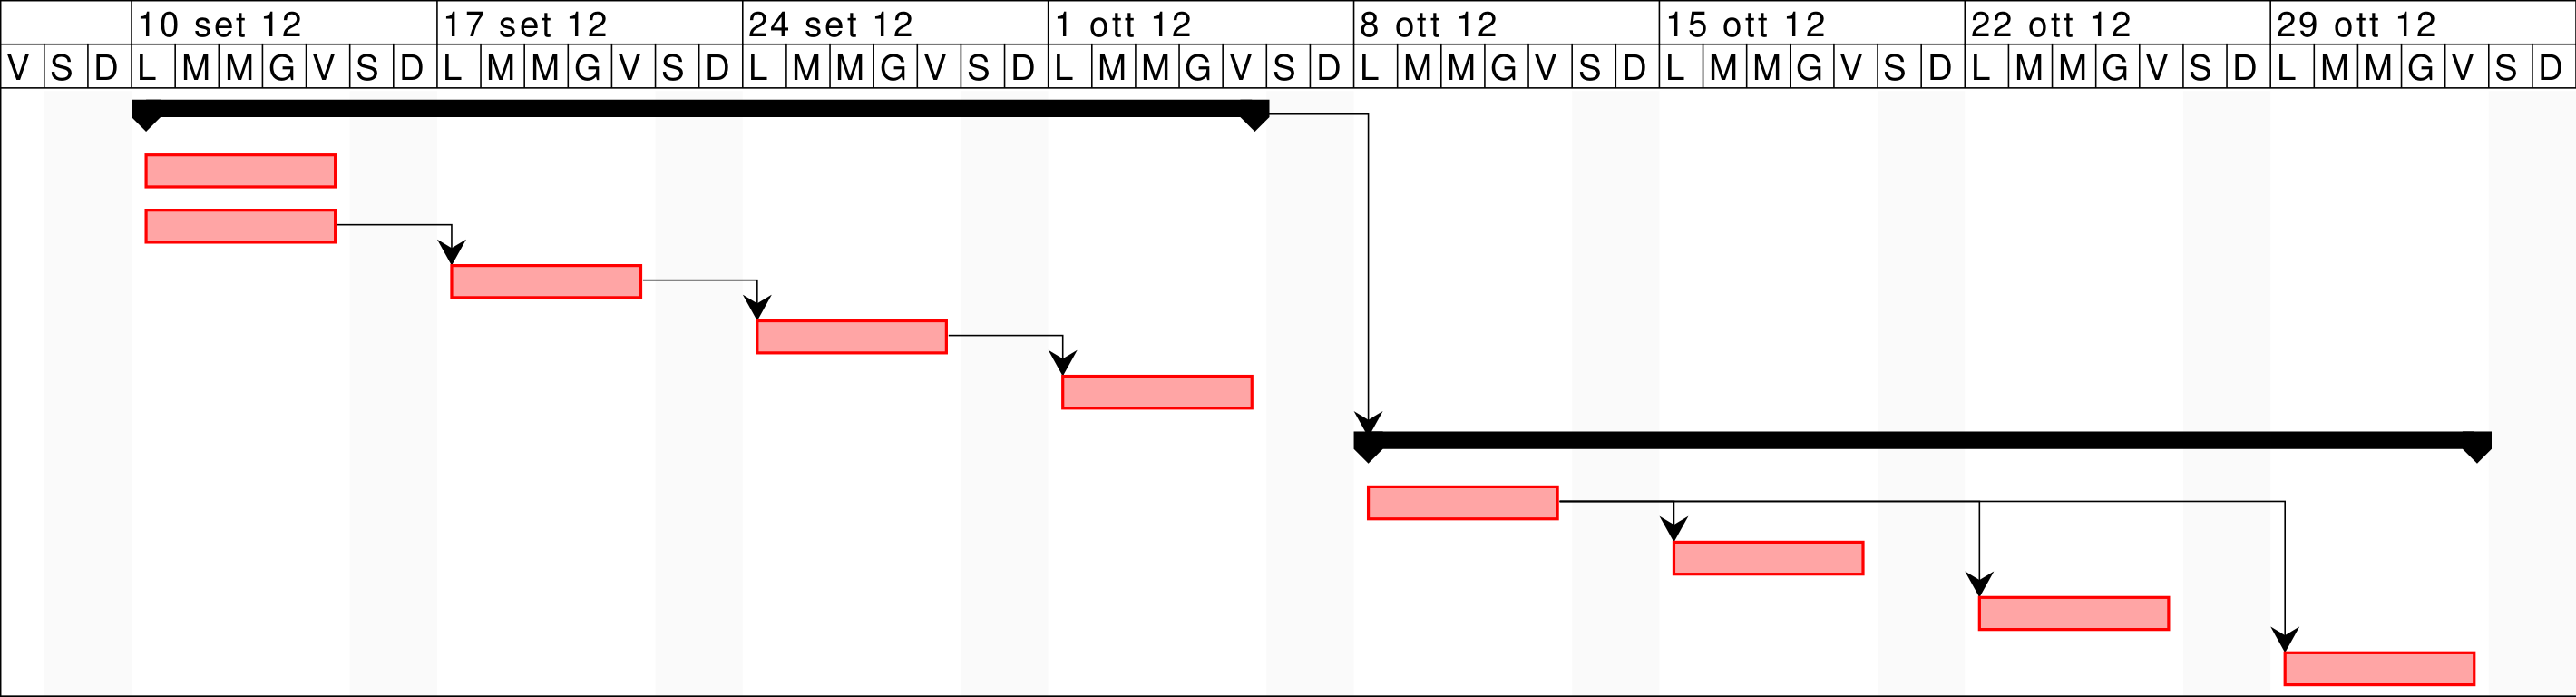
\includegraphics[width=14.5cm]{gantt.png}
		\label{fig:tesi:stage:gantt}
		\caption{Diagramma di Gantt}
	\end{center}
	\end{figure}

	\section{Norme di stage}
	
	\subsection{Ambiente di lavoro}
	Nel corso dello stage sono stati impiegati diversi strumenti per gestire le attività di progetto e produrre la documentazione prevista.
	
	\begin{table}[ht]
	\centering
	\begin{tabular}{|l|l|}
	\hline
	\textsc{Controllo di versione} & \underline{Mercurial} 2.0.2 \\ \hline
	\textsc{Editor \LaTeX} & \underline{LaTeXila} 2.4.0 - \underline{gedit} 3.4.0 con \textit{gedit-latex-plugin} \\ \hline
	\textsc{Editor UML} & \underline{UMLet} 11.5.1 \\ \hline
	\textsc{Foglio elettronico} & \underline{LibreOffice Calc} 3.6 \\ \hline
	\textsc{Gestione database} & \underline{MySQL Workbench} 5.2.42 \\ \hline
	\textsc{Mockup} & \underline{Pencil} 2.0.2 \\	\hline
	\textsc{Pianificazione} & \underline{ProjectLibre} 1.5.1 \\ \hline
	\textsc{Repository} & \underline{Bitbucket} \\ \hline
	\textsc{Sistema operativo} & \underline{Ubuntu} 12.04 \\ \hline
	\end{tabular}
	\caption{Configurazione dell'ambiente di lavoro}
	\label{tab:tesi:stage:norme:strumenti}
	\end{table}

	\subsection{Documentazione}
	La documentazione è stata redatta in \LaTeX e pubblicata in formato \underline{PDF}.
	
	\paragraph{Struttura}
	Ciascun documento presenta una struttura e un formato comuni:
	\begin{enumerate}
		\item il frontespizio riporta il titolo del documento, l'autore e la data di compilazione;
		\item la seconda pagina mostra una sintetica e sommaria presentazione dello scopo del documento;
		\item la terza pagina riporta il registro delle modifiche;
		\item la quarta pagina mostra l'indice del documento;
		\item a seguire è visibile la lista delle figure e delle tabelle presenti nel documento.
	\end{enumerate}
	
	\paragraph{Registro delle modifiche}
	Il registro delle modifiche tiene traccia della cronologia delle versioni del documento (dalla più recente alla più vecchia), mostrando per ciascuna di esse la data di redazione e una descrizione sintetica delle modifiche apportate.

	\paragraph{Versionamento}
	A ciascun documento è stato assegnato un numero di versione $x.y$, ove $x$ rappresenta l'ultima \textsc{versione formale}, rivista e approvata dal referente aziendale e disponibile a terze parti interessate (membri del team di progetto, tutor interno), mentre $y$ indica una \textsc{versione preliminare} ad uso interno, eventualmente consultabile dal referente aziendale.

	Un incremento del numero di versione secondario $y$ occorre a seguito dell'aggiunta o integrazione dei contenuti o di una revisione informale di tutto o parte del documento.

	Un incremento del numero di versione primario $x$ si verifica solamente in seguito alla revisione formale e all'approvazione del documento da parte del referente aziendale.

	\paragraph{Nomi dei file}
	Il nome assegnato alle versioni preliminari di ciascun documento contiene esclusivamente caratteri alfabetici minuscoli, eventualmente separati mediante il simbolo '-' (trattino). Le versioni formali aggiungono un suffisso, formato dal simbolo '\textunderscore' (trattino basso) e dal numero di versione $x.y$.

	\subsection{Modello relazionale}
	Il modello relazionale del database è stato realizzato mediante lo strumento adottato dal team di progetto, ossia l'editor \textit{MySQL Workbench}, per facilitare la condivisione e l'integrazione delle informazioni. I file e gli script generati utilizzan la codifica \underline{UTF-8} per garantire la massima compatibilità.
	
	\paragraph{Nomi delle tabelle}
	I nomi delle tabelle sono espressi in lingua italiana e contengono solo caratteri alfabetici minuscoli e non accentati, eventualmente separati mediante il simbolo '\textunderscore' (trattino basso).
	
	\paragraph{Nomi degli attributi}
	I nomi degli attributi sono espressi in lingua italiana e contengono solo caratteri alfabetici in formato \underline{CamelCase}, ove la lettera iniziale è sempre in minuscolo.
	
	\subsection{Digrammi UML}
	Durante l'attività di stage sono stati redatti e inclusi nella documentazione diversi diagrammi dei casi d'uso, dei package e delle classi secondo lo standard \underline{UML} 2.x. Nei paragrafi successivi vengono presentate le linee guida e le convenzioni concernenti la struttura e il formato.
	
	\paragraph{Casi d'uso} La notazione utilizzata per identificare un caso d'uso è così definita:
	$$UC.x.y$$
	ove:
	\begin{itemize}
		\item $UC$ è l'abbreviazione di \textit{Use Case} (Caso d'uso);
		\item $x \in \left\{1,2,\ldots\right\}$ è il numero identificativo del diagramma cui appartiene il caso d'uso;
		\item $y \in \left\{1,2,\ldots\right\}$ è il numero associato al caso d'uso.
	\end{itemize}
	
	\paragraph{Package}
	I nomi dei package contengono solo caratteri alfabetici minuscoli e non accentati, eventualmente separati dal carattere '-' (trattino).
	
	\paragraph{Classi}
	I nomi delle classi sono in formato \textit{CamelCase} e le sottoclassi riportano per esteso o in forma abbreviata l'identificatore della superclasse diretta: nel secondo caso sono presenti - come prefisso - le sole lettere maiuscole, nel medesimo ordine di apparizione.
	
	\subsection{Requisiti funzionali} I requisiti del sistema software sono univocamente identificati mediante la seguente notazione:
	$$Rf.x.y$$
	ove:
	\begin{itemize}
		\item $Rf$ è l'abbreviazione di \textit{requisito funzionale};
		\item $x \in \left\{ob,de\right\}$ rappresenta il tipo di requisito funzionale (\textit{ob} per obbligatorio, \textit{de} per desiderabili);
		\item $y \in \left\{1,2,\ldots\right\}$ è il numero associato ad un requisito.
	\end{itemize}
	
	\subsubsection{Tracciamento dei casi d'uso}
	Il tracciamento delle dipendenze tra casi d'uso e requisiti software è stato realizzato mediante il foglio elettronico , ove:
	\begin{itemize}
	   \item ciascuna riga rappresenta un requisito del sistema software;
	   \item ciascuna colonna rappresenta un caso d'uso;
	   \item ciascuna cella contiene il carattere 'X' se esiste una relazione di dipendenza tra il caso d'uso e il requisito, altrimenti è vuota.
	 \end{itemize}
	 
  Per ciascuna riga e colonna viene impiegata una semplice formula per asserire la completezza e la necessità della matrice dei requisiti:  
  \begin{center}
    \texttt{CONTA.SE(A:Z;"X")}   
  \end{center}
  ove:
  \begin{itemize}
    \item \texttt{A:Z} corrisponde all'intervallo di celle di una singola riga o colonna;
    \item \texttt{"X"} rappresenta il pattern da cercare (nello specifico, una stringa di lunghezza unitaria);
    \item \texttt{CONTA.SE} è una funzione a due argomenti (intervallo di celle, pattern) che restituisce il numero di celle nell'intervallo indicato contenenti una o più occorrenze del pattern specificato.
  \end{itemize}
  
	\paragraph{Completezza} Per ogni colonna, se la formula restituisce un valore pari a 0 (zero) sta ad indicare che il requisito utente non è soddisfatto da alcun requisito software.
	
	\paragraph{Necessità} Per ogni riga, se la formula restituisce un valore pari a 0 (zero) sta ad indicare che il requisito software corrispondente è superfluo.

	\section{Fase 1: criterio di classificazione}
	\label{sec:tesi:stage:fase-1}
	Il patrimonio di conoscenza della piattaforma è garantito essenzialmente dai contenuti pubblicati dagli utenti ed arricchito dal loro valore informativo: ciascuno di essi, a prescindere dalla forma (testo, immagini, audio, video, \ldots) o dalla classe (domanda, discorso, evento, recensione, \ldots), trasmette delle informazioni inerenti uno o più elementi del dominio tematico della piattaforma.
	
	\begin{figure}[ht]
     \begin{center}
       
\includegraphics{placeholder.png}
       \label{fig:tesi:stage:classificazione:serbatoio-contenuti}
       \caption{Contenuti informativi e conoscenza}
     \end{center}
   \end{figure}
   
   Allo state attuale, la piattaforma si limita ad essere un immenso serbatoio di contenuti informativi disaggregati, priva della capacità di classificare e catalogare il sapere in essa custodito per conferirvi una struttura ordinata, una sorta di indice enciclopedico in grado di rendere tale sapere facilmente fruibile e consultabile.
  
  Il primo passo consiste nell'osservare come ciascun contenuto rappresenti - dal punto di vista conoscitivo - un insieme di frammenti di informazioni, ciascuno dei quali contribuisce ad arricchire il sapere relativo a qualche \textsc{entità} (astratta o concreta), che rappresenta oggetto di discussione all'interno del dominio della piattaforma.
  
	\begin{figure}[ht]
     \begin{center}
       
\includegraphics{placeholder.png}
       \label{fig:tesi:stage:fase-uno:contenuti-informativi}
       \caption{Valore informativo di un contenuto}
     \end{center}
   \end{figure}
  
  L'insieme di entità definite - in un certo istante - all'interno della piattaforma ne costituisce il \textsc{dominio della conoscenza} (di seguito per brevità \textsc{dominio}), analogamente all'insieme di lemmi di un'enciclopedia. Ciascun frammento di informazione identificabile in un contenuto è concettualmente associabile e riferibile ad uno o più entità di tale dominio.
  
  L'obiettivo primario del nuovo criterio di classificazione consiste dunque nel modellare tale dominio e le relazioni esistenti tra le relative entità ed i contenuti informativi. 

	\begin{figure}[ht]
     \begin{center}
       
\includegraphics{placeholder.png}
       \label{fig:tesi:stage:fase-uno:dominio-conoscenza}
       \caption{Dominio di conoscenza della piattaforma}
     \end{center}
   \end{figure}
   
  \subsection{Entità}
  
  \subsection{Etichette}
  
  \subsubsection{Accezioni}

  \subsubsection{Sinonimi}
  
  \subsection{Contenuti}
  
  \begin{itemize}
    \item metafora dell'enciclopedia
    \item approcci dell'utente all'esplorazione
  \end{itemize}

	\section{Fase 2: interfaccia grafica}
	\label{sec:tesi:stage:fase-2}
	
	\subsection{Analisi dei requisiti}
	
	\subsection{Progettazione}

	% CHAPTER
	\chapter{Valutazioni finali}
	\label{ch:tesi:valutazioni}

	\section{Consuntivo}

	\section{Competenze professionali}
	\begin{itemize}
	\item multidisciplinarietà: coinvolgimento di figure professionali provenienti da numerosi e variegati settori professionali (psicologia, sociologia, marketing, economia, informatica, ingegneria, \ldots)
	\end{itemize}

	\section{Stage e università}

	% APPENDIX
	\appendix
	\chapter[Glossario]{Glossario}
	\label{ch:appendice:glossario}
	
	\section*{B}
	\paragraph{Bitbucket - \url{https://bitbucket.org/}} \hfill \\
	Piattaforma web per la gestione delle attività di progetto con supporto a strumenti di controllo di versione distribuito.

	\section*{C}
	\paragraph{CamelCase} \hfill \\
	Convenzione per la scrittura di espressioni composte unendo le parole tra loro e mantenendo ciascuna iniziale in maiuscolo.
	
	\paragraph{Chilometri zero} \hfill \\
	Filosofia di consumo basata sull'acquisto di beni agroalimentari direttamente dal produttore, evitando la filiera, tutelando l'ambiente e valorizzando la produzione locale del territorio.

	\section*{G}
	\paragraph{gedit - \url{http://projects.gnome.org/gedit/}} \hfill \\
	Editor di testo ufficiale dell'ambiente desktop GNOME.
	\paragraph{Gruppi di acquisto} \hfill \\
	Insieme (stabile o provvisorio) di consumatori che acquista mediante ordine collettivo un consistente numero di beni direttamente dal produttore, spesso per conseguire prezzi vantaggiosi o ammortizzare eventuali spese accessorie.
	
	\section*{L}
	\paragraph{LaTeXila - \url{http://projects.gnome.org/latexila/}} \hfill \\
	Editor LaTex integrato per l'ambiente desktop GNOME.
	\paragraph{LibreOffice Calc - \url{http://www.libreoffice.org/}} \hfill \\
  Applicazione per fogli di calcolo della suite di produttività \textit{LibreOffice}.

	\section*{M}
	\paragraph{Mercurial - \url{http://mercurial.selenic.com/}} \hfill \\
	Strumento multi piattaforma, gratuito ed open source per il controllo di versione distribuito.
	\paragraph{MySQL Workbench - \url{http://www.mysql.it/products/workbench/}} \hfill \\
	Applicazione multi piattaforma, gratuita ed open source per la progettazione, lo sviluppo e l'amministrazione di database MySQL. 

	\section*{P}
	\paragraph{PDF (Portable Document Format)} \hfill \\
	Formato di file per la rappresentazione di documenti in maniera indipendente dalla piattaforma hardware e software.
	\paragraph{Pencil - \url{http://pencil.evolus.vn/}} \hfill \\
	Applicazione multi piattaforma, gratuita ed open source per la realizzazione di prototipi di interfacce grafiche.
	\paragraph{ProjectLibre - \url{http://sourceforge.net/projects/projectlibre/}} \hfill \\
	Applicazione multi piattaforma, gratuita ed open source per il \textit{project management}, che consente di realizzare diagrammi di Gantt e di PERT, gestire le risorse allocate e le attività pianificate, \ldots\ .

	\section*{R}
	\paragraph{Rete sociale} \hfill \\
	Insieme di persone, aventi interessi in comune e inclini a collaborare e condividere idee o informazioni, e di relazioni di tipo esperienziale definite tra tali soggetti.

	\section*{U}
	\paragraph{Ubuntu - \url{http://www.ubuntu.com/}} \hfill \\
	Distribuzione Linux gratuita derivata da Debian.
	\paragraph{UML (Unified Modelling Laanguage) - \url{http://www.uml.org/}} \hfill \\
	Standard internazionale per un linguaggio di modellazione, che definisce un insieme di notazioni grafiche per la rappresentazione visiva di sistemi.
	\paragraph{UMLet - \url{http://www.umlet.com/}} \hfill \\
	Applicazione multi piattaforma, gratuita ed open source per la realizzazione di diagrammi UML.
	\paragraph{UTF-8 (Unicode Transformation Format-8) - \url{http://www.unicode.org/standard/}} \hfill \\
	Codifica dei caratteri Unicode a 8 bit. Si distingue dalla maggior parte delle altre codifiche per la capacità di rappresentare un insieme più ampio di caratteri, non limitato ad una specifica area geografica o alfabeto.

\end{document}
